%email an gerhard.kniewasser@student.tugraz.at

% **************************************************************************************************
% ** SPSC Report and Thesis Template
% **************************************************************************************************
%
% ***** Authors *****
% Daniel Arnitz, Paul Meissner, Stefan Petrik
% Signal Processing and Speech Communication Laboratory (SPSC)
% Graz University of Technology (TU Graz), Austria
%
% ***** Changelog *****
% 0.1   2010-01-25   extracted from report template by Daniel Arnitz (not ready yet)
% 0.2   2010-02-08   added thesis titlepage and modified layout (not ready yet)
% 0.3   2010-02-18   added TUG logo and statutory declaration
% 0.4   2010-02-18   moved the information fields below % **************************************************************************************************
% ** SPSC Report and Thesis Template
% **************************************************************************************************
%
% ***** Authors *****
% Daniel Arnitz, Paul Meissner, Stefan Petrik
% Signal Processing and Speech Communication Laboratory (SPSC)
% Graz University of Technology (TU Graz), Austria
%
% ***** Changelog *****
%
% ***** Todo *****
%
% **************************************************************************************************



\documentclass[%
a4paper,% !!! ATTENTION: geometry package below !!!
\Twosided,% !!! ATTENTION: geometry package below !!!
openany,% begin chapters with new right page (openright) or don't care (openany)
11pt,%
fleqn,% equations not centered, but on the left side
tablecaptionbelow,% captions below tables
% titlepage,% use title
pointlessnumbers,% do not generate point at the end of section numbers (e.g. 1.4.5 instead of 1.4.5.)
final,%
]{scrreprt}% (KOMA)

\usepackage[paper=a4paper,\Twosided,%
textheight=246mm,%
textwidth=160mm,%
heightrounded=true,% round textheight to multiple of lines (avoids overfull vboxes)
ignoreall=true,% do not include header, footer, and margins in calculations
marginparsep=5pt,% marginpar only used for signs (centered), thus only small sep. needed
marginparwidth=10mm,% prevent margin notes to be out of page
hmarginratio=2:1,% set margin ration (inner:outer for twoside) - (2:3 is default)
]{geometry}%


% master
\usepackage{ifthen}% for optional parts
\usepackage[utf8]{inputenc}% German special characters
\ifthenelse{\equal{\DocumentLanguage}{en}}{\usepackage[USenglish]{babel}}{}%
\ifthenelse{\equal{\DocumentLanguage}{de}}{\usepackage[ngerman]{babel}}{}%
\usepackage[%
headtopline,plainheadtopline,% activate all lines (header and footer)
headsepline,plainheadsepline,%
footsepline,plainfootsepline,%
footbotline,plainfootbotline,%
automark% auto update \..mark
]{scrpage2}% (KOMA)
\usepackage{makeidx}% used to make an index directory
\usepackage[]{caption}% customize captions
\usepackage{multicol}%
\usepackage[stable,bottom,hang,splitrule,multiple,symbol*]{footmisc}% customize footnotes


% text
\usepackage{varioref}% improved references
\usepackage{color}% e.g., for color boxes
\usepackage{rotating}% to rotate objects
\usepackage{gensymb}% symbols (perthousand, Celsius, ...)
\usepackage[right]{eurosym}% euro symbol on the right side (51 EUR)
\usepackage[normalem]{ulem}% cross-out, strike-out, underlines (normalem: keep \emph italic)
%\usepackage[safe]{textcomp}% loading in safe mode to avoid problems (see LaTeX companion)
%\usepackage[geometry,misc]{ifsym}% technical symbols
\usepackage{remreset}%\@removefromreset commands (e.g., for continuous footnote numbering)
\usepackage[%
breaklinks=true,% allow line break in links
colorlinks=true,% if false: framed link
linkcolor=black,anchorcolor=black,citecolor=black,filecolor=black,%
menucolor=black,urlcolor=black]{hyperref}% hyperlinks for references


% math
\usepackage{amsmath,amssymb,amstext,bm} % use math packages
\usepackage{mathcomp}% symbols (perthousand, ...) in math mode


% graphics
\usepackage{graphicx}% use simple graphics
\usepackage{subfigure}% subfigures (a),(b),(c)... within figures
\usepackage{flafter}% place floats always after reference
\usepackage{placeins}% preventing floats from crossing a barrier
\usepackage{float}% to place floats !HERE!
\usepackage{psfrag}% replace text in eps figures


% tables
\usepackage{hhline}% hline doesn't work with colored columns, so using hhline
\usepackage{longtable}% for tables longer than one page
\usepackage{dcolumn}% for number alignment in tables
\usepackage{colortbl}% color in tables


% listings
%\usepackage{alltt}% verbatim environment with commands available
\usepackage{listings}% program code listings


% other
%\usepackage{layout}% graphical page layout (spacings)
\usepackage{xspace}% add space after macros if not followed by punctuation character
\makeindex% used for index creation

 (encoding...)
% 0.5   2010-03-02   added \ShortTitle to fix problems with long thesis titles
%                    added \ThesisType (makes the template suitable for MSc, BSc, PhD, ... Thesis)
%
% ***** Todo *****
% - Introduction/Usage
% **************************************************************************************************

% **************************************************************************************************
% basic setup
\newcommand{\DocumentType}{report} % "thesis" / "report"
\newcommand{\DocumentLanguage}{de} % "en" / "de"
\newcommand{\Twosided}{} % "twoside" / ""


% **************************************************************************************************
% template setup -- do not change these unless you know what you are doing!
% **************************************************************************************************
% ** SPSC Report and Thesis Template
% **************************************************************************************************
%
% ***** Authors *****
% Daniel Arnitz, Paul Meissner, Stefan Petrik
% Signal Processing and Speech Communication Laboratory (SPSC)
% Graz University of Technology (TU Graz), Austria
%
% ***** Changelog *****
%
% ***** Todo *****
%
% **************************************************************************************************



\documentclass[%
a4paper,% !!! ATTENTION: geometry package below !!!
\Twosided,% !!! ATTENTION: geometry package below !!!
openany,% begin chapters with new right page (openright) or don't care (openany)
11pt,%
fleqn,% equations not centered, but on the left side
tablecaptionbelow,% captions below tables
% titlepage,% use title
pointlessnumbers,% do not generate point at the end of section numbers (e.g. 1.4.5 instead of 1.4.5.)
final,%
]{scrreprt}% (KOMA)

\usepackage[paper=a4paper,\Twosided,%
textheight=246mm,%
textwidth=160mm,%
heightrounded=true,% round textheight to multiple of lines (avoids overfull vboxes)
ignoreall=true,% do not include header, footer, and margins in calculations
marginparsep=5pt,% marginpar only used for signs (centered), thus only small sep. needed
marginparwidth=10mm,% prevent margin notes to be out of page
hmarginratio=2:1,% set margin ration (inner:outer for twoside) - (2:3 is default)
]{geometry}%


% master
\usepackage{ifthen}% for optional parts
\usepackage[utf8]{inputenc}% German special characters
\ifthenelse{\equal{\DocumentLanguage}{en}}{\usepackage[USenglish]{babel}}{}%
\ifthenelse{\equal{\DocumentLanguage}{de}}{\usepackage[ngerman]{babel}}{}%
\usepackage[%
headtopline,plainheadtopline,% activate all lines (header and footer)
headsepline,plainheadsepline,%
footsepline,plainfootsepline,%
footbotline,plainfootbotline,%
automark% auto update \..mark
]{scrpage2}% (KOMA)
\usepackage{makeidx}% used to make an index directory
\usepackage[]{caption}% customize captions
\usepackage{multicol}%
\usepackage[stable,bottom,hang,splitrule,multiple,symbol*]{footmisc}% customize footnotes


% text
\usepackage{varioref}% improved references
\usepackage{color}% e.g., for color boxes
\usepackage{rotating}% to rotate objects
\usepackage{gensymb}% symbols (perthousand, Celsius, ...)
\usepackage[right]{eurosym}% euro symbol on the right side (51 EUR)
\usepackage[normalem]{ulem}% cross-out, strike-out, underlines (normalem: keep \emph italic)
%\usepackage[safe]{textcomp}% loading in safe mode to avoid problems (see LaTeX companion)
%\usepackage[geometry,misc]{ifsym}% technical symbols
\usepackage{remreset}%\@removefromreset commands (e.g., for continuous footnote numbering)
\usepackage[%
breaklinks=true,% allow line break in links
colorlinks=true,% if false: framed link
linkcolor=black,anchorcolor=black,citecolor=black,filecolor=black,%
menucolor=black,urlcolor=black]{hyperref}% hyperlinks for references


% math
\usepackage{amsmath,amssymb,amstext,bm} % use math packages
\usepackage{mathcomp}% symbols (perthousand, ...) in math mode


% graphics
\usepackage{graphicx}% use simple graphics
\usepackage{subfigure}% subfigures (a),(b),(c)... within figures
\usepackage{flafter}% place floats always after reference
\usepackage{placeins}% preventing floats from crossing a barrier
\usepackage{float}% to place floats !HERE!
\usepackage{psfrag}% replace text in eps figures


% tables
\usepackage{hhline}% hline doesn't work with colored columns, so using hhline
\usepackage{longtable}% for tables longer than one page
\usepackage{dcolumn}% for number alignment in tables
\usepackage{colortbl}% color in tables


% listings
%\usepackage{alltt}% verbatim environment with commands available
\usepackage{listings}% program code listings


% other
%\usepackage{layout}% graphical page layout (spacings)
\usepackage{xspace}% add space after macros if not followed by punctuation character
\makeindex% used for index creation


\input{./base/layout_\DocumentType}
% **************************************************************************************************
% ** SPSC Report and Thesis Template
% **************************************************************************************************
%
% ***** Authors *****
% Daniel Arnitz, Paul Meissner, Stefan Petrik
% Signal Processing and Speech Communication Laboratory (SPSC)
% Graz University of Technology (TU Graz), Austria
%
% ***** Changelog *****
%
% ***** Todo *****
%
% **************************************************************************************************



% **************************************************************************************************
% * SECTIONING AND TEXT
% **************************************************************************************************

% new chapter, section, ... plus a few addons
%   part
\newcommand{\newpart}[2]{\FloatBarrier\cleardoublepage\part{#1}\label{part:#2}}%
%   chapter
\newcommand{\newchapter}[2]{\FloatBarrier\chapter{#1}\label{chp:#2}}
\newcommand{\newchapterNoTOC}[2]{\FloatBarrier\stepcounter{chapter}\chapter*{#1}\label{chp:#2}}%
%   section
\newcommand{\newsection}[2]{\FloatBarrier\vspace{5mm}\section{#1}\label{sec:#2}}%
\newcommand{\newsectionNoTOC}[2]{\FloatBarrier\vspace{5mm}\stepcounter{section}\section*{#1}\label{sec:#2}}%
%   subsection
\newcommand{\newsubsection}[2]{\FloatBarrier\vspace{3mm}\subsection{#1}\label{sec:#2}}%
\newcommand{\newsubsectionNoTOC}[2]{\FloatBarrier\vspace{3mm}\stepcounter{subsection}\subsection*{#1}\label{sec:#2}}%
%   subsubsection
\newcommand{\newsubsubsection}[2]{\vspace{2mm}\subsubsection{#1}\label{sec:#2}}%
\newcommand{\newsubsubsectionNoTOC}[2]{\vspace{2mm}\stepcounter{subsubsection}\subsubsection*{#1}\label{sec:#2}}%

% next paragraph
\newcommand{\nxtpar}{\par\bigskip}

% "stylish" quotes on the right side
\newcommand{\openingquote}[2]{\hfill\parbox[t]{10cm}{\itshape\raggedleft{"#1"}\\\footnotesize -- #2}\nxtpar}%

% direct quotes
% \newenvironment{directquote}{\nxtpar\hrule}{\hrule}\hfill\litref{#1}{#2}}

% warnings and attention signs in marginpar
\newcommand{\MDanger}{\marginpar{\Huge\centering\fbox{\textbf{!}}}}%
\newcommand{\MAttention}{\marginpar{\Huge\centering\textbf{!}}}%
\newcommand{\MHint}{\marginpar{\Huge\centering\textbf{\checkmark}}}%
\newcommand{\MQuestion}{\marginpar{\Huge\centering\textbf{?}}}%

% same footnote number as last one
\newcommand{\lastfootnotemark}{\addtocounter{footnote}{-1}\footnotemark}%

% value-unit commands (for 457 kHz, etc)
\newcommand{\vu}[2]{\mbox{$#1\,\text{#2}$}} % "value~unit" ... prevents e.g. 456 \linebreak mV
\newcommand{\vuc}[3]{\mbox{$#1\,\text{#2}\;#3\,\%$}} % "value~unit~tolerance-per-cent"
\newcommand{\vum}[3]{\mbox{$#1\,\text{#2}\;#3\,\perthousand$}} % "value~unit~tolerance-per-mil"

% reminders
\newcommand{\reminder}[1]{\colorbox{red}{#1}\xspace}%
\newcommand{\rem}{\reminder{(...)}}%
\newcommand{\remq}{\reminder{???}}%
\newcommand{\uc}{\nxtpar\colorbox{yellow}{... under construction ...}\nxtpar}%

% misc
\newcommand{\pwd}{.} % present working directory (can be used to create relativ paths per part, etc.)


% **************************************************************************************************
% * MATH
% **************************************************************************************************

% highlighting
\newcommand{\vm}[1]{\bm{#1}}% vector or matrix

% operators
\newcommand{\E}[1]{\text{E}\!\left\{#1\right\}}% expectation operator
\newcommand{\var}[1]{\text{var}\!\left\{#1\right\}}% variance operator
\renewcommand{\ln}[1]{\text{ln}\!\left(#1\right)}% natural logarithm
\newcommand{\ld}[1]{\text{ld}\!\left(#1\right)}% logarithm base 2
\renewcommand{\log}[1]{\text{log}\!\left(#1\right)}% logarithm (base 10)
\newcommand{\logb}[2]{\text{log}_{#1}\!\left(#2\right)}% logarithm base ...
\newcommand{\avgvar}[1]{\overline{\text{var}}\!\left\{#1\right\}}% average variance operator
\renewcommand{\Re}[1]{\text{Re}\!\left\{#1\right\}}% real part
\renewcommand{\Im}[1]{\text{Im}\!\left\{#1\right\}}% imaginary part

% other
\newcommand{\conj}{^\ast}% conjugate complex
\newcommand{\mtx}[2]{\left[\begin{array}{#1}#2\end{array}\right]}%vector/matrix


% **************************************************************************************************
% * FLOATS (FIGURES, TABLES, LISTINGS, ...)
% **************************************************************************************************

% figures without frames
%   standard
\newcommand{\fig}[3]{\begin{figure}\centering\includegraphics[width=\textwidth]{#1}\caption{#2}\label{fig:#3}\end{figure}}%
%   with controllable parameters
\newcommand{\figc}[4]{\begin{figure}\centering\includegraphics[#1]{#2}\caption{#3}\label{fig:#4}\end{figure}}%
%   two subfigures
\newcommand{\twofig}[6]{\begin{figure}\centering%
\subfigure[#2]{\includegraphics[width=0.495\textwidth]{#1}}%
\subfigure[#4]{\includegraphics[width=0.495\textwidth]{#3}}%
\caption{#5}\label{fig:#6}\end{figure}}%
%   two subfigures and controllable parameters
\newcommand{\twofigc}[8]{\begin{figure}\centering%
\subfigure[#3]{\includegraphics[#1]{#2}}%
\subfigure[#6]{\includegraphics[#4]{#5}}%
\caption{#7}\label{fig:#8}\end{figure}}%

% framed figures
%   standard
\newcommand{\figf}[3]{\begin{figure}\centering\fbox{\includegraphics[width=\textwidth]{#1}}\caption{#2}\label{fig:#3}\end{figure}}%
%   with controllable parameters
\newcommand{\figcf}[4]{\begin{figure}\centering\fbox{\includegraphics[#1]{#2}}\caption{#3}\label{fig:#4}\end{figure}}%
%   two subfigures
\newcommand{\twofigf}[6]{\begin{figure}\centering%
\fbox{\subfigure[#2]{\includegraphics[width=0.495\textwidth]{#1}}}%
\fbox{\subfigure[#4]{\includegraphics[width=0.495\textwidth]{#3}}}%
\caption{#5}\label{fig:#6}\end{figure}}%
%   two subfigures and controllable parameters
\newcommand{\twofigcf}[8]{\begin{figure}\centering%
\fbox{\subfigure[#3]{\includegraphics[#1]{#2}}}%
\fbox{\subfigure[#6]{\includegraphics[#4]{#5}}}%
\caption{#7}\label{fig:#8}\end{figure}}%

% listings
\newcommand{\filelisting}[4]{\lstinputlisting[print=true,language=#1,caption={#3},label={lst:#4}]{#2}}

% preserve backslash for linebreaks in tables (ragged... redefines \\, thus it has to be preserved)
\newcommand{\pbs}[1]{\let\temp=\\#1\let\\=\temp}%

\graphicspath{{./drawings/}{./plots/}{./images/}}
% **************************************************************************************************
% ATTENTION: Make sure that makeindex is set to -s "./base/index.sty"
% **************************************************************************************************

% uncomment to get watermarks:
% \usepackage[first,bottom,light,draft]{draftcopy}
% \draftcopyName{ENTWURF}{160}


% **************************************************************************************************
% information fields

% general
\newcommand{\DocumentTitle}{Image Processing and Pattern Recognition}
\newcommand{\DocumentSubtitle}{Assignment 1}
\newcommand{\ShortTitle}{BVME Assignment 1} % used in headers (keep short!)
\newcommand{\DocumentAuthor}{Stefan Nöhmer (0830668)}
\newcommand{\DocumentDate}{Graz, \today}
%    for thesis only (will be ignored for reports)
\newcommand{\ThesisType}{Master's Thesis}
\newcommand{\Organizations}{Signal Processing and Speech Communications Laboratory \\ Graz University of Technology \\[1cm] on behalf of \\ Some Company} % SPSC \\ TUG \\[1cm] on behalf of \\ A Nice Company
\newcommand{\Advisors}{Dipl.-Ing. Dr. Assoc.Prof. Klaus Witrisal \\ Dipl.-Ing. Paul Meissner} % Advisor 1 \\ Advisor 2 \\ ...
\newcommand{\Supervisors}{Univ.-Prof. Dipl.-Ing. Dr.techn. Gernot Kubin}

% revision number
\newcommand{\RevPrefix}{alpha~}
\newcommand{\RevLarge}{1}
\newcommand{\RevSmall}{1}

% confidential?
\newcommand{\ConfidNote}{confidential}% {"confidential", "eyes only", ...}

% short command for vectors
\newcommand{\vect}[1]{\mathbf{#1}}


\begin{document}

%listingstyle:
\definecolor{orange}{rgb}{0.75,0.65,0}
\definecolor{gruen}{rgb}{0,0.5,0}
\definecolor{listinggray}{gray}{0.97}
\definecolor{listingshadow}{gray}{0.2}
\lstloadlanguages{Matlab}
\lstset{frame=shadowbox,
		rulesepcolor=\color{listingshadow},
		numbers=left,
		basicstyle=\scriptsize\ttfamily,
		numberstyle=\tiny,
		keywordstyle=\color{blue}\bfseries, % bold black keywords
		identifierstyle=, % nothing happens
		commentstyle=\color{gruen}, % comments
		stringstyle=\color{orange}, % typewriter type for strings
		showstringspaces=false,
		tabsize=4,
		backgroundcolor=\color{listinggray}
        }

% **************************************************************************************************
% titlepage
\input{./base/titlepage_\DocumentType}

% statutory declaration for theses
\ifthenelse{\equal{\DocumentType}{thesis}}{% **************************************************************************************************
% ** SPSC Report and Thesis Template
% **************************************************************************************************
%
% ***** Authors *****
% Daniel Arnitz, Paul Meissner, Andreas Laesser, Stefan Petrik
% Signal Processing and Speech Communication Laboratory (SPSC)
% Graz University of Technology (TU Graz), Austria
%
% ***** Changelog *****
% 0.1   2010-02-18   created
% 0.2   2010-03-02   added German declaration
%
% ***** Todo *****
% **************************************************************************************************

\cleardoublepage
\pagestyle{empty}\pagenumbering{roman}

\vspace*{1cm}

% English
\ifthenelse{\equal{\DocumentLanguage}{en}}{
\begin{center}\Large\bfseries Statutory Declaration\end{center}\vspace*{1cm}
\noindent I declare that I have authored this thesis independently, that I have not used other than the declared sources$/$resources, and that I have explicitly marked all material which has been quoted either literally or by content from the used sources.
\par\vspace*{4cm}
\centerline{
\begin{tabular}{m{1.5cm}cm{1.5cm}m{3cm}m{1.5cm}cm{1.5cm}}
\cline{1-3} \cline{5-7}
 & date & & & & (signature) &\\
\end{tabular}}
}

% German
\ifthenelse{\equal{\DocumentLanguage}{de}}{
\begin{center}\Large\bfseries Eidesstattliche Erkl�rung\end{center}\vspace*{1cm}
Ich erkl�re an Eides statt, dass ich die vorliegende Arbeit selbstst�ndig verfasst, andere als die angegebenen Quellen$/$Hilfsmittel nicht benutzt, und die den benutzten Quellen w�rtlich und inhaltlich entnommene Stellen als solche kenntlich gemacht habe.
\par\vspace*{4cm}
\centerline{
\begin{tabular}{m{1.5cm}cm{1.5cm}m{3cm}m{1.5cm}cm{1.5cm}}
\cline{1-3} \cline{5-7}
 & Graz, am & & & & (Unterschrift) &\\
\end{tabular}}
}

}{}


% **************************************************************************************************
% **************************************************************************************************
% user-defined part

\chapter{Task 1: Interpolation}

In diesem Task sollten 3 unterschiedliche Algorithmen für die Interpolation eines rotierten Bildes implementiert und untersucht werden. Die Berechnung ist prinzipiell die gleiche wie in der händischen Version:

\begin{equation}
 \begin{bmatrix} y_{in} \\ x_{in} \end{bmatrix} = R^{-1} \begin{bmatrix} y_{out} \\ x_{out} \end{bmatrix}
\end{equation}

\begin{equation}
 R = \begin{bmatrix} cos \varphi & -sin \varphi \\ sin \varphi & cos \varphi \end{bmatrix} \; \; \Rightarrow R^{-1} = \begin{bmatrix} cos \varphi & sin \varphi \\ -sin \varphi & cos \varphi \end{bmatrix}
\end{equation}

Diese Koordinatentransformation übernimmt die Funktion \texttt{task1\_transform}.

Die Rotation selbst übernehmen die Funktionen \texttt{task1\_rotate\_nn}, \texttt{task1\_rotate\_bilinear} und \texttt{task1\_rotate\_bicubic}.
Da in Matlab der Koordinatenursprung (1,1) immer links oben im Bild liegt, muss dieser rechnerisch in die Bildmitte verschoben werden, um die Rotation um den Bildmittelpunkt auszuführen.

Mit jedem der 3 Algorithmen wird das Bild schrittweise um -10°, -10° und 20° gedreht. Dadurch entsteht nach diesen 3 Rotationen wieder das Originalbild, jedoch mit teilweise schwarzen Pixel. Diese entstehen dadurch, dass Pixel außerhalb des Eingangsbildes als 0 gewertet werden, und durch die Rotation ins Ausgabebild wandern.

Nach den 3 Rotationen wird das Bild mit dem Originalbild verglichen, indem die PSNR berechnet wird. Dazu muss der MSE berechnet werden, dieser sollte jedoch für die schwarzen, hereinrotierten Pixel ignoriert werden. Dies geschieht durch eine Maske, die für alle Bilder gleich ist, um eine vergleichbare PSNR für alle Bilder zu erhalten. Da alle Pixel innerhalb der Maske nicht von schwarzen, hereinrotierten Pixel beeinflusst werden sollen, wird die Maske für die Interpolation mit den weitreichendsten Auswirkungen der außenliegenden Pixel berechnet (die bikubische Interpolation). Dazu wird ein weißes Bild (alle Pixel sind 1) 3 mal rotiert, und dann sämtliche Pixel, die nicht mehr 1 sind wegmaskiert. Diese Maske wird dann bei jeder MSE-Berechnung durch die Funktion \texttt{task1\_mse} berücksichtigt.

Bei der Berechnung der PSNR wurde als Maximalwert der Pixel der Wert 1 verwendet, da dieser in \texttt{double}-Darstellung der höchste vorkommende Wert ist.

Das Matlab-Skript \texttt{task1.m} führt sämtliche Berechnungen für diesen Task durch, zeigt die Ergebnisbilder an und gibt die jeweilige PSNR aus.

Abbildung~\ref{fig:t1_original} zeigt das Eingangsbild, mit dem die Berechnungen durchgeführt wurden.

\begin{figure}[htb]
 \centering
 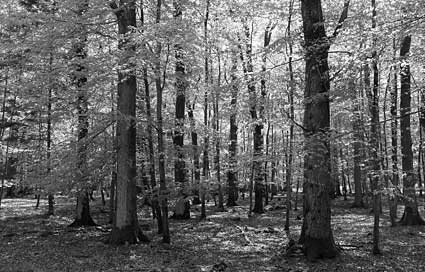
\includegraphics{./img/t1_original.png}
 \caption{Das Eingangsbild für alle Interpolationen in Task 1}
 \label{fig:t1_original}
\end{figure}

Der Matlab-Code aller Skripte und Funktionen befindet sich ebenfalls im Anhang.

\clearpage


\section{Nearest Neighbor Interpolation}

Bei der Nearest Neighbor Interpolation wird der Pixelwert des Ausgabebildes durch den nächstgelegenen Pixel des Eingangsbildes gebildet. Das geschieht, indem einfach die Pixelkoordinaten auf den nächstgelegenen Integerwert gerundet werden. In Matlab wird dazu die Funktion \texttt{round} verwendet.

Der Algorithmus durchläuft alle Pixel des Ausgabebildes, berechnet die dazugehörigen exakten Pixelkoordinaten des Eingangsbildes, und rundet diese auf den nächsten Pixel.

\begin{equation}
 I_{out}(y_{out}, x_{out}) = I_{in}(round(y_{in}), round(x_{in}))
\end{equation}

Dadurch leidet die Qualität des Ergebnisses, weil eigentlich keine richtige Interpolation statt findet. Es wird nur der nächstgelegene Pixelwert verwendet, was unter anderem bei Kanten im Bild falsche Werte liefern kann. Durch die Einfachheit dieses Algorithmus ist er jedoch im Vergleich zu den anderen schnell.


\smallskip

Abbildung~\ref{fig:t1_nn} zeigt, das Ergebnis der Nearest Neighbor Interpolation. Man kann die falsch interpolierten Pixel gut erkennen, die durch die Wahl eines einzelnen Pixels entstehen (statt der Berechnung aus mehreren umliegenden Pixel). Die erreichte PSNR war 15.474dB.

\begin{figure}[htb]
 \centering
 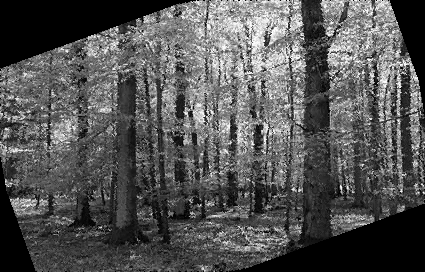
\includegraphics{./img/t1_nn.png}
 \caption{Das Ergebnis für Nearest Neighbor Interpolation in Task 1}
 \label{fig:t1_nn}
\end{figure}

\clearpage



\section{Bilineare Interpolation}
\label{t1_bl}

Bei der bilinearen Interpolation wird nicht mehr nur ein Pixel betrachtet, sondern die 4 naheliegendsten Pixel zu den berechneten Pixelkoordinaten (diese 4er-Nachbarschaft ist auf der händischen Berechnung zu Task 1 skizziert). Die umliegenden Pixel werden dabei mit der Distanz zu den berechneten Pixelkoordinaten gewichtet und aufsummiert. Die dazu verwendete Gewichtsfunktion $g(x)$ ist in der Aufgabenstellung angegeben, wobei x die Distanz zwischen exakten Pixelkoordinaten und dem tatsächlichen Pixel ist.

Der Algorithmus erstellt für das gesamte Bild zwei Matrizen, in denen die Pixelkoordinaten in x- bzw. y-Richtung gespeichert sind (Matlab-Funktion \texttt{meshgrid}). Jetzt wird das gesamte Bild durchlaufen, und für jeden Pixel die exakten Koordinaten berechnet. Aus diesen exakten Koordinaten und den Koordinatenmatrizen werden dann 2 Matrizen berechnet, die die Abstände aller Pixel zu den exakten Koordinaten enthalten. Diese Matrizen werden dann der Gewichtsfunktion \texttt{task1\_g} übergeben, welche daraus 2 Gewichtsmatrizen berechnet. Diese werden miteinander und mit dem Eingangsbild multipliziert, um alle gewichteten Pixel zu erhalten (die meisten dieser Pixel sind 0). Summiert man nun über die gesamte Matrix, so erhält man den interpolierten Wert für den aktuellen Pixel.
Diese Methode ist zwar einfach verständlich und übersichtlich, da aber die meisten Pixel 0 sind und dadurch bei der Berechnung wegfallen ist sie nicht effizient und hat eine lange Laufzeit. Sie beinhaltet aber bereits auch schon die Behandlung der außenliegenden Pixel, die dadurch einfach 0 gewertet werden, wodurch eine spezielle Randbehandlung überflüssig ist. Außerdem kann sie auch für die bikubische Interpolation (und auch andere Interpolationen) verwendet werden, wenn man einfach die Gewichtsfunktion \texttt{task1\_g} durch eine andere ersetzt.


\smallskip

Abbildung~\ref{fig:t1_bl} zeigt das Ergebnis der bilinearen Interpolation. Man erkennt, dass die Kanten im Bild nun viel glätter wirken, da die Ausgabepixel immer aus den 4 umliegenden Pixel berechnet werden. Allerdings entsteht durch diese Berechnung auch eine geringe Unschärfe gegenüber dem Originalbild. Durch die zusätzlichen Berechnungen ist die Laufzeit wesentlich länger als bei der Nearest Neighbor Interpolation. Die erreichte PSNR war 15.5438dB, und damit höher als bei der Nearest Neighbor Interpolation. Das liegt an der genaueren Berechnung des Pixelwertes aus den umliegenden Pixel, anstatt einfach nur den nächsten Pixel zu verwenden.

\begin{figure}[htb]
 \centering
 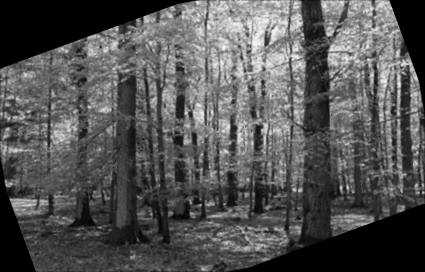
\includegraphics{./img/t1_bl.png}
 \caption{Das Ergebnis für bilineare Interpolation in Task 1}
 \label{fig:t1_bl}
\end{figure}

\clearpage



\section{Bikubische Interpolation}

Ähnlich der bilinearen Interpolation berechnet die bikubische Interpolation den Wert eine Pixels aus den den exakten Pixelkoordinaten umliegenden Pixelwerten. Anders als bei der bilinearen Interpolation werden hier jedoch nicht nur die 4 umliegenden Pixel, sondern 16 umliegende Pixel betrachtet. Diese werden dann mit einem Polynom gewichtet, dessen Koeffizienten variiert werden können um das Ergebnis zu beeinflussen. Bei schlechten Koeffizienten kann es bei der bikubischen Interpolation jedoch zu Ringing-Effekten (sichtbare ``Schwingungen'') kommen. Bei den hier verwendeten Koeffizienten entsteht jedoch ein schärfer wirkendes Bild.

Der Algorithmus ist gleich implementiert wie die bilineare Interpolation (siehe Abschnitt~\ref{t1_bl}). Der einzige Unterschied ist die Verwendung einer anderen Gewichtsfunktion \texttt{task1\_h}, welche nicht nach der Entfernung zu den exakten Pixelkoordinaten gewichtet, sondern je nach Entfernung ein Polynom berechnet. So werden mehrere Werte in der Gewichtsmatrix (die 16-er Nachbarschaft) ungleich 0 und für die Berechnung des Pixels verwendet. Da auch hier wieder viele Pixel in den Gewichtsmatrizen 0 sind, ist die Variante auch ineffizient (aber einfach) implementiert.

\smallskip

Abbildung~\ref{fig:t1_bc} zeigt das Ergebnis der bikubischen Interpolation. Im Vergleich zur bilinearen Interpolation ist das Ergebnis noch besser, die Unschärfe hat abgenommen. Durch das eingeführte Polynom als Gewichtsfunktion wirkt das Ausgabebild nochmals besser als bei der bilinearen Interpolation. Gleich wie bei der bilinearen Interpolation ist die Laufzeit auch wesentlich länger als bei der Nearest Neighbor Interpolation.

Die erreichte PSN war 15.542dB, also etwas niedriger als bei der bilinearen Interpolation. Das könnte durch einen Fehler in der Implementierung entstehen, welcher aber vor Abgabeschluss nicht mehr gefunden werden konnte. Optisch sieht das Ergebnis der bikubischen Interpolation besser aus, deswegen wäre es naheliegend, dass die PSNR ebenfalls höher ist.

\begin{figure}[htb]
 \centering
 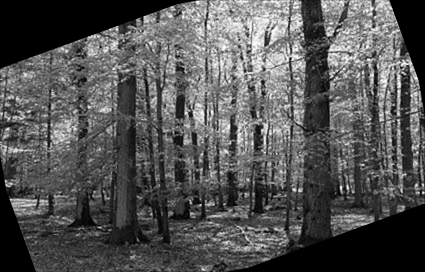
\includegraphics{./img/t1_bc.png}
 \caption{Das Ergebnis für bikubische Interpolation in Task 1}
 \label{fig:t1_bc}
\end{figure}

\clearpage



\chapter{Task 2: Denoising}

blah blah



% **************************************************************************************************
% **************************************************************************************************

%\appendix
%\bibliographystyle{/.base/ieeetran}
%\bibliography{_bibliography}

% place all floats and create label on last page
\FloatBarrier\label{end-of-document}
\end{document}

